\documentclass[../../General.tex]{subfiles}
\begin{document}

\section{Diseño de subsistema de tracción y dirección}

\subsection{Descripción general del subsistema}

El subsistema de tracción y dirección está representado en la Figura \ref{fig:SubsistemaTraslacion}. El movimiento principal del vehículo permite el avance lineal mediante tracción en el eje posterior y la maniobrabilidad de viraje mediante un mecanismo de dirección orientable tipo Ackermann independiente en el eje frontal.


\begin{figure}[H]
	\captionsetup{justification=raggedright, singlelinecheck=false, labelsep=none}
	\caption[Vista isométrica y frontal del Subsistema de tracción y dirección.]{} 
	\textit{Vista isométrica y frontal del Subsistema de tracción y dirección.} \par\medskip
	
	\begin{minipage}{0.5\textwidth}
		\centering
		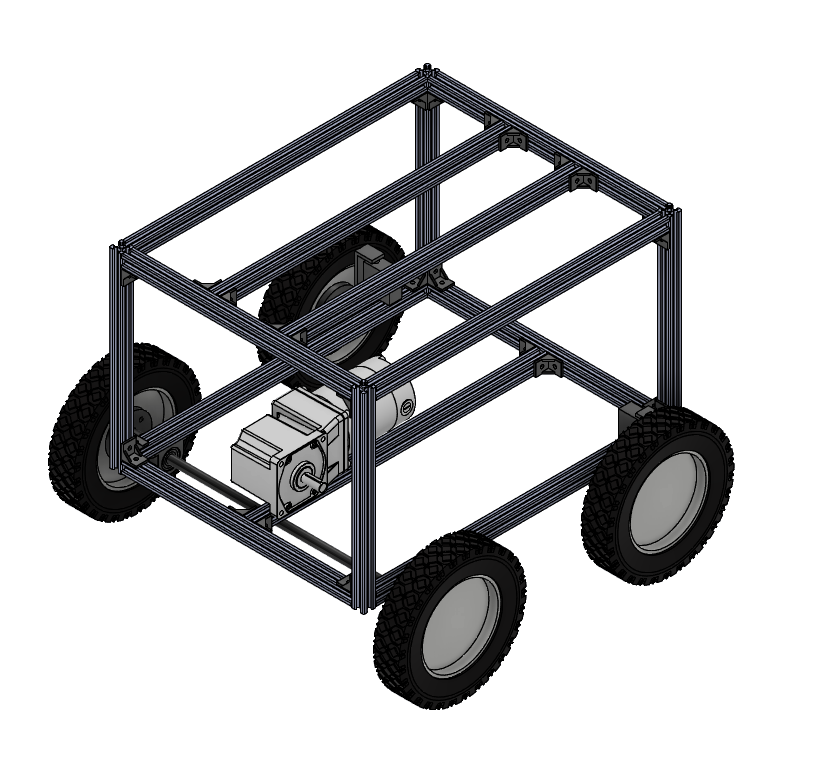
\includegraphics[width=\linewidth]{Recursos/Imagenes/ImagenesDisenoMecanico/MECANISMO_TRACCION.png}
	\end{minipage}\hfill
	\begin{minipage}{0.5\textwidth}
		\centering
		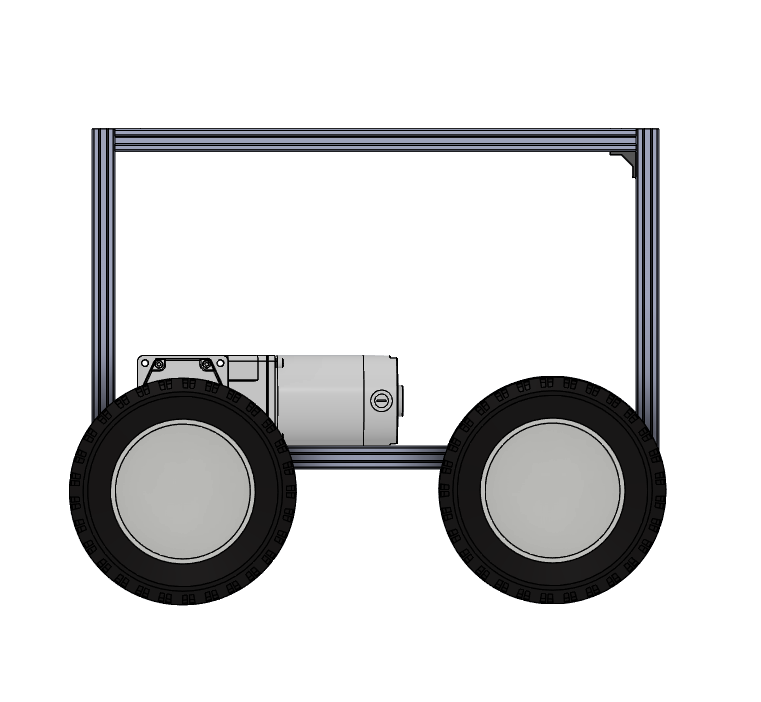
\includegraphics[width=\linewidth]{Recursos/Imagenes/ImagenesDisenoMecanico/MECANISMO_TRACCION_SIDE.png}
	\end{minipage}
	\par\medskip
	
	\raggedright
	\footnotesize \textit{Nota.} Elaboración propia.
	\label{fig:SubsistemaTraslacion}
\end{figure}

\subsection{Planteamiento inicial y parámetros de diseño}

Para definir estrictamente las exigencias dinámicas del subsistema motriz durante la traslación y viraje, se consolida en primera instancia el balance de masa integral del vehículo. La masa operativa se divide sistemáticamente, donde la batería de potencia de química ión de litio asume $3.00\text{ kg}$, el hardware electrónico acoplado y los tendidos de cableado representan $2.38\text{ kg}$, la instrumentación óptica meteorológica en conjunto con la computadora de procesamiento suman $0.98\text{ kg}$, y la carcasa estructural protectora de aluminio envuelve $3.50\text{ kg}$. Por el lado cinemático, el cuadrilátero de elevación añade $1.55\text{ kg}$, la plataforma de orientación suma $1.30\text{ kg}$ y el tren de rodadura constituido por ejes macizos y neumáticos incorpora $4.79\text{ kg}$. En sumatoria, se ratifica una masa nominal de trabajo del sistema estandarizada en $17.50\text{ kg}$. Si se consideran los márgenes de contingencia por accesorios adicionales o depósitos de polvo, la masa crítica de sobrecarga pericial asciende a $20.00\text{ kg}$. 

Al evaluar la geometría de estabilidad dinámica de esta configuración masiva en el espacio tridimensional, un ancho de vía seleccionado de $380\text{ mm}$ y una distancia entre ejes de $450\text{ mm}$ determinan una ubicación central simétrica del centro de gravedad, el cual se sitúa a $180\text{ mm}$ del nivel del piso. Este modelado asegura matemáticamente un ángulo de vuelco lateral de $46.5^\circ$, otorgando una estabilidad estática infalible y blindando al robot móvil frente al riesgo de volteo al recorrer terrenos y pasillos irregulares con pendientes severas de hasta $15^\circ$. Complementando la marcha en terrenos angostos, la arquitectura de dirección independiente basada en la geometría Ackermann asegura de manera algorítmica que, al demandar un giro límite de la rueda interna de $35.0^\circ$, la mangueta de la rueda exterior pivotee en concordancia un ángulo de $23.8^\circ$, logrando un trazado de curva perfecto que ofrece un radio mínimo de viraje en el eje posterior de $0.83\text{ m}$.

\begin{center}
    \footnotesize
    \begin{xltabular}{\textwidth}{|p{3.5cm}|>{\centering\arraybackslash}p{2.5cm}|>{\centering\arraybackslash}p{2.5cm}|>{\centering\arraybackslash}X|}
        \caption{Parámetros, variables y restricciones del subsistema de tracción y dirección Ackermann\label{tab:parametros_diseno_ackermann}} \\
        \hline
        \rowcolor[HTML]{D9E1F2} 
        Parámetro o Variable & Símbolo & Valor o Límite & Descripción \\ \hline
        \endfirsthead
        
        \multicolumn{4}{c}%
        {\tablename\ \thetable{} -- Continuación de la página anterior} \\
        \hline
        \rowcolor[HTML]{D9E1F2} 
        Parámetro o Variable & Símbolo & Valor o Límite & Descripción \\ \hline
        \endhead
        
        \hline
        \endfoot
        
        \hline
        \endlastfoot
        
        Masa total del robot & $m$ & $17.50\text{ kg}$ a $20.00\text{ kg}$ & Masa combinada del chasis, baterías, sensores y mecanismos articulados. \\ \hline
        Aceleración de la gravedad & $g$ & constante $9.81\text{ m/s}^2$ & Aceleración gravitacional local. \\ \hline
        Peso total del robot & $W$ & $171.66\text{ N}$ a $196.20\text{ N}$ & Fuerza gravitacional total expresada por el peso. \\ \hline
        Radio efectivo de rueda & $r$ & $0.10\text{ m}$ & Radio de los neumáticos de tracción y dirección. \\ \hline
        Ancho de vía o track width & $b$ & $380\text{ mm}$ & Distancia transversal entre los pivotes de dirección del eje frontal. \\ \hline
        Distancia entre ejes o wheelbase & $L$ & $450\text{ mm}$ & Distancia longitudinal entre el eje frontal orientable y el eje posterior fijo. \\ \hline
        Altura del centro de masa & $h_{cm}$ & $180\text{ mm}$ & Elevación vertical del centro de gravedad respecto al suelo. \\ \hline
        Posición longitudinal del CG & $L_{cm}$ & $225\text{ mm}$ & Ubicación horizontal del centro de gravedad medida desde el eje posterior. \\ \hline
        Radio del parche de contacto & $r_c$ & $25\text{ mm}$ & Radio equivalente de la huella de contacto neumático y suelo. \\ \hline
        Radio de frotamiento & $e$ & $15\text{ mm}$ & Distancia entre el centro de la huella del neumático y la proyección del pivote. \\ \hline
        Brazo de palanca de la mangueta & $L_{\text{mangueta}}$ & $30\text{ mm}$ & Distancia perpendicular desde el pivote de dirección a la articulación del actuador. \\ \hline
        Velocidad lineal del robot & $v$ & $1.0\text{ m/s}$ & Velocidad tangencial de avance en el eje longitudinal local. \\ \hline
        Aceleración lineal & $a$ & $0.50\text{ m/s}^2$ & Aceleración longitudinal máxima requerida en el despegue o cambio de marcha. \\ \hline
        Ángulo de rueda interior & $\delta_i$ & $35.0^\circ$ & Ángulo de viraje de la rueda delantera interna a la curva. \\ \hline
        Ángulo de rueda exterior & $\delta_o$ & $23.8^\circ$ & Ángulo de viraje de la rueda delantera externa a la curva. \\ \hline
        Ángulo de dirección medio virtual & $\delta$ & $28.5^\circ$ & Ángulo equivalente de dirección en el centro geométrico del eje frontal. \\ \hline
        Radio de giro al centro del eje & $R$ & $0.83\text{ m}$ & Distancia desde el centro del eje posterior al Centro Instantáneo de Rotación. \\ \hline
        Pendiente del terreno & $\beta$ & $15.0^\circ$ & Inclinación del plano de marcha respecto a la horizontal. \\ \hline
        Coeficiente de rodadura & $f_r$ & $0.06$ & Factor de resistencia por deformación del neumático sobre terreno suelto o grava. \\ \hline
        Coeficiente de fricción estática & $\mu_s$ & $0.70$ & Adherencia estática entre el caucho del neumático y la superficie del suelo. \\ \hline
        Reacciones normales del suelo & $N_f, N_r$ & $N_f = 61.63\text{ N}, N_r = 104.18\text{ N}$ & Cargas normales ejercidas por el suelo sobre el eje frontal y posterior. \\ \hline
        Fuerza de tracción total & $F_{\text{trac}}$ & $54.38\text{ N}$ cont. a $63.13\text{ N}$ arr. & Fuerza tangencial requerida en el eje posterior para vencer la pendiente y rodadura. \\ \hline
        Torque de pivoteo por mangueta & $\tau_{\text{piv}}$ & $0.951\text{ N}\cdot\text{m}$ Nom. a $1.087\text{ N}\cdot\text{m}$ Crít. & Momento de resistencia al giro en reposo de cada rueda delantera. \\ \hline
        Relación de reducción & $i_t, i_s$ & $i_t = 1.0\text{ directa}, i_s = 1.0\text{ directo}$ & Relación de transmisión de la caja para tracción y dirección. \\ \hline
        Eficiencia de transmisión & $\eta_t, \eta_s$ & $\eta_t = 0.85, \eta_s = 0.90$ & Rendimiento mecánico del tren de tracción y del mecanismo de dirección. \\ \hline
        Factor de seguridad & $S$ & $1.30$ & Margen de diseño para absorber sobrecargas dinámicas e irregularidades. \\ \hline
        Torque motor de tracción & $T_{\text{motor},t}$ & $8.32\text{ N}\cdot\text{m}$ Nom. a $9.51\text{ N}\cdot\text{m}$ Crít. & Torque continuo requerido en el eje del motorreductor de tracción. \\ \hline
        Torque por servomotor de dirección & $T_{\text{servo}}$ & $1.374\text{ N}\cdot\text{m}$ Nom. a $1.571\text{ N}\cdot\text{m}$ Crít. & Torque requerido individualmente en cada uno de los dos servomotores de dirección. \\ \hline
        Inercia del tren de tracción & $J_{\text{ruedas}}$ & $0.024\text{ kg}\cdot\text{m}^2$ & Inercia de rotación equivalente de los componentes giratorios del tren de tracción. \\ \hline
        Fricción estática de tracción & $T_{s,t}$ & $0.40\text{ N}\cdot\text{m}$ & Torque de fricción estática inicial en el tren motriz posterior. \\ \hline
        Inercia de mangueta & $J_{\text{mang}}$ & $1.2 \times 10^{-3}\text{ kg}\cdot\text{m}^2$ & Momento de inercia rotacional de la mangueta y neumático delantero. \\ \hline
        Aceleración angular de viraje & $\ddot{\delta}$ & $10.5\text{ rad/s}^2$ & Aceleración angular de viraje impuesta por el servomotor al pivotar la rueda. \\ \hline
        Fricción estática de dirección & $T_{s,s}$ & $0.10\text{ N}\cdot\text{m}$ & Torque de fricción estática inicial en el pivote de dirección y servomotor. \\ \hline
	\end{xltabular}
\end{center}

Siguiendo los criterios de modelado descritos por Siegwart en 2004 \citep{siegwart2004mobile} y la teoría de terramecánica de Wong \citep{wong2022ground}, se asume lo siguiente:
\begin{enumerate}
    \item Todos los componentes del bastidor y la estructura principal actúan como un cuerpo rígido indeformable en el plano de movimiento \citep{gillespie1992vehicle}. [COMENTARIO: TENER EN CUENTA LO QUE PASARÍA SI NO SE TOMA ESTA SUPOSICIÓN, QUÉ CAMBIARÍA? APRENDE QUÉ PASA PARA PODER RESPONDER.]
    \item Las ruedas operan bajo condiciones de rodadura pura en la dirección de marcha y sin deslizamiento transversal instantáneo en el punto de contacto con el suelo.
    \item Las ruedas del eje frontal giran ángulos diferenciados de forma que sus líneas de centro, extendidas junto con el eje posterior, concurren en un único Centro Instantáneo de Rotación.
    \item La masa total del robot se distribuye de manera simétrica respecto al plano medio longitudinal, concentrando las variaciones de carga dinámica en el plano de ordenadas al subir pendientes.
\end{enumerate}

\subsection{Planteamiento cinemático y estático}

Con base en el modelo cinemático para robots móviles publicado por Siegwart, para lograr un viraje suave y exento de deslizamiento lateral en los neumáticos en el plano horizontal, los ejes de rotación de todas las ruedas deben intersectarse en un único Centro Instantáneo de Rotación, el cual se ubica sobre la extensión del eje posterior fijo. Esto exige que la rueda delantera interior gire un ángulo mayor que la rueda exterior, cumpliendo la relación geométrica estricta de la condición fundamental de Ackermann \citep{siegwart2004mobile, jazar2017vehicle}:

\begin{equation*}
    \cot \delta_o - \cot \delta_i = \frac{b}{L}
\end{equation*}

Donde la variable $b$ representa la distancia transversal entre los pivotes verticales y $L$ la distancia entre ejes.

Definiendo $R$ como la distancia desde el Centro Instantáneo de Rotación hasta el centro del eje posterior, el ángulo de dirección equivalente virtual en el centro del eje frontal cumple:

\begin{equation*}
    \tan \delta = \frac{L}{R}
\end{equation*}

Los ángulos de viraje específicos para la rueda interior y exterior resultan en:

\begin{equation*}
    \delta_i = \arctan \left[ \frac{L}{R - \frac{b}{2}} \right]
\end{equation*}

\begin{equation*}
    \delta_o = \arctan \left[ \frac{L}{R + \frac{b}{2}} \right]
\end{equation*}

El radio mínimo de giro utilizable por el robot queda limitado por el ángulo de giro mecánico máximo de la mangueta interior:

\begin{equation*}
    R_{\min} = \frac{L}{\tan \delta_{i,\max}} + \frac{b}{2}
\end{equation*}

Para evitar que las ruedas posteriores arrastren o desgasten la superficie en virajes, las velocidades angulares de las ruedas traseras interna y externa deben ser:

\begin{equation*}
    \omega_{r,i} = \frac{v}{r} \left[ 1 - \frac{b}{2R} \right], \quad \omega_{r,o} = \frac{v}{r} \left[ 1 + \frac{b}{2R} \right]
\end{equation*}

\begin{figure}[H]
	\captionsetup{justification=raggedright, singlelinecheck=false, labelsep=none}
	
	\caption[Diagrama de cuerpo libre de movimiento del subsistema de tracción.]{} 
	
	\textit{Diagrama de cuerpo libre de movimiento del subsistema de tracción.} \par\medskip
	
	\centering
	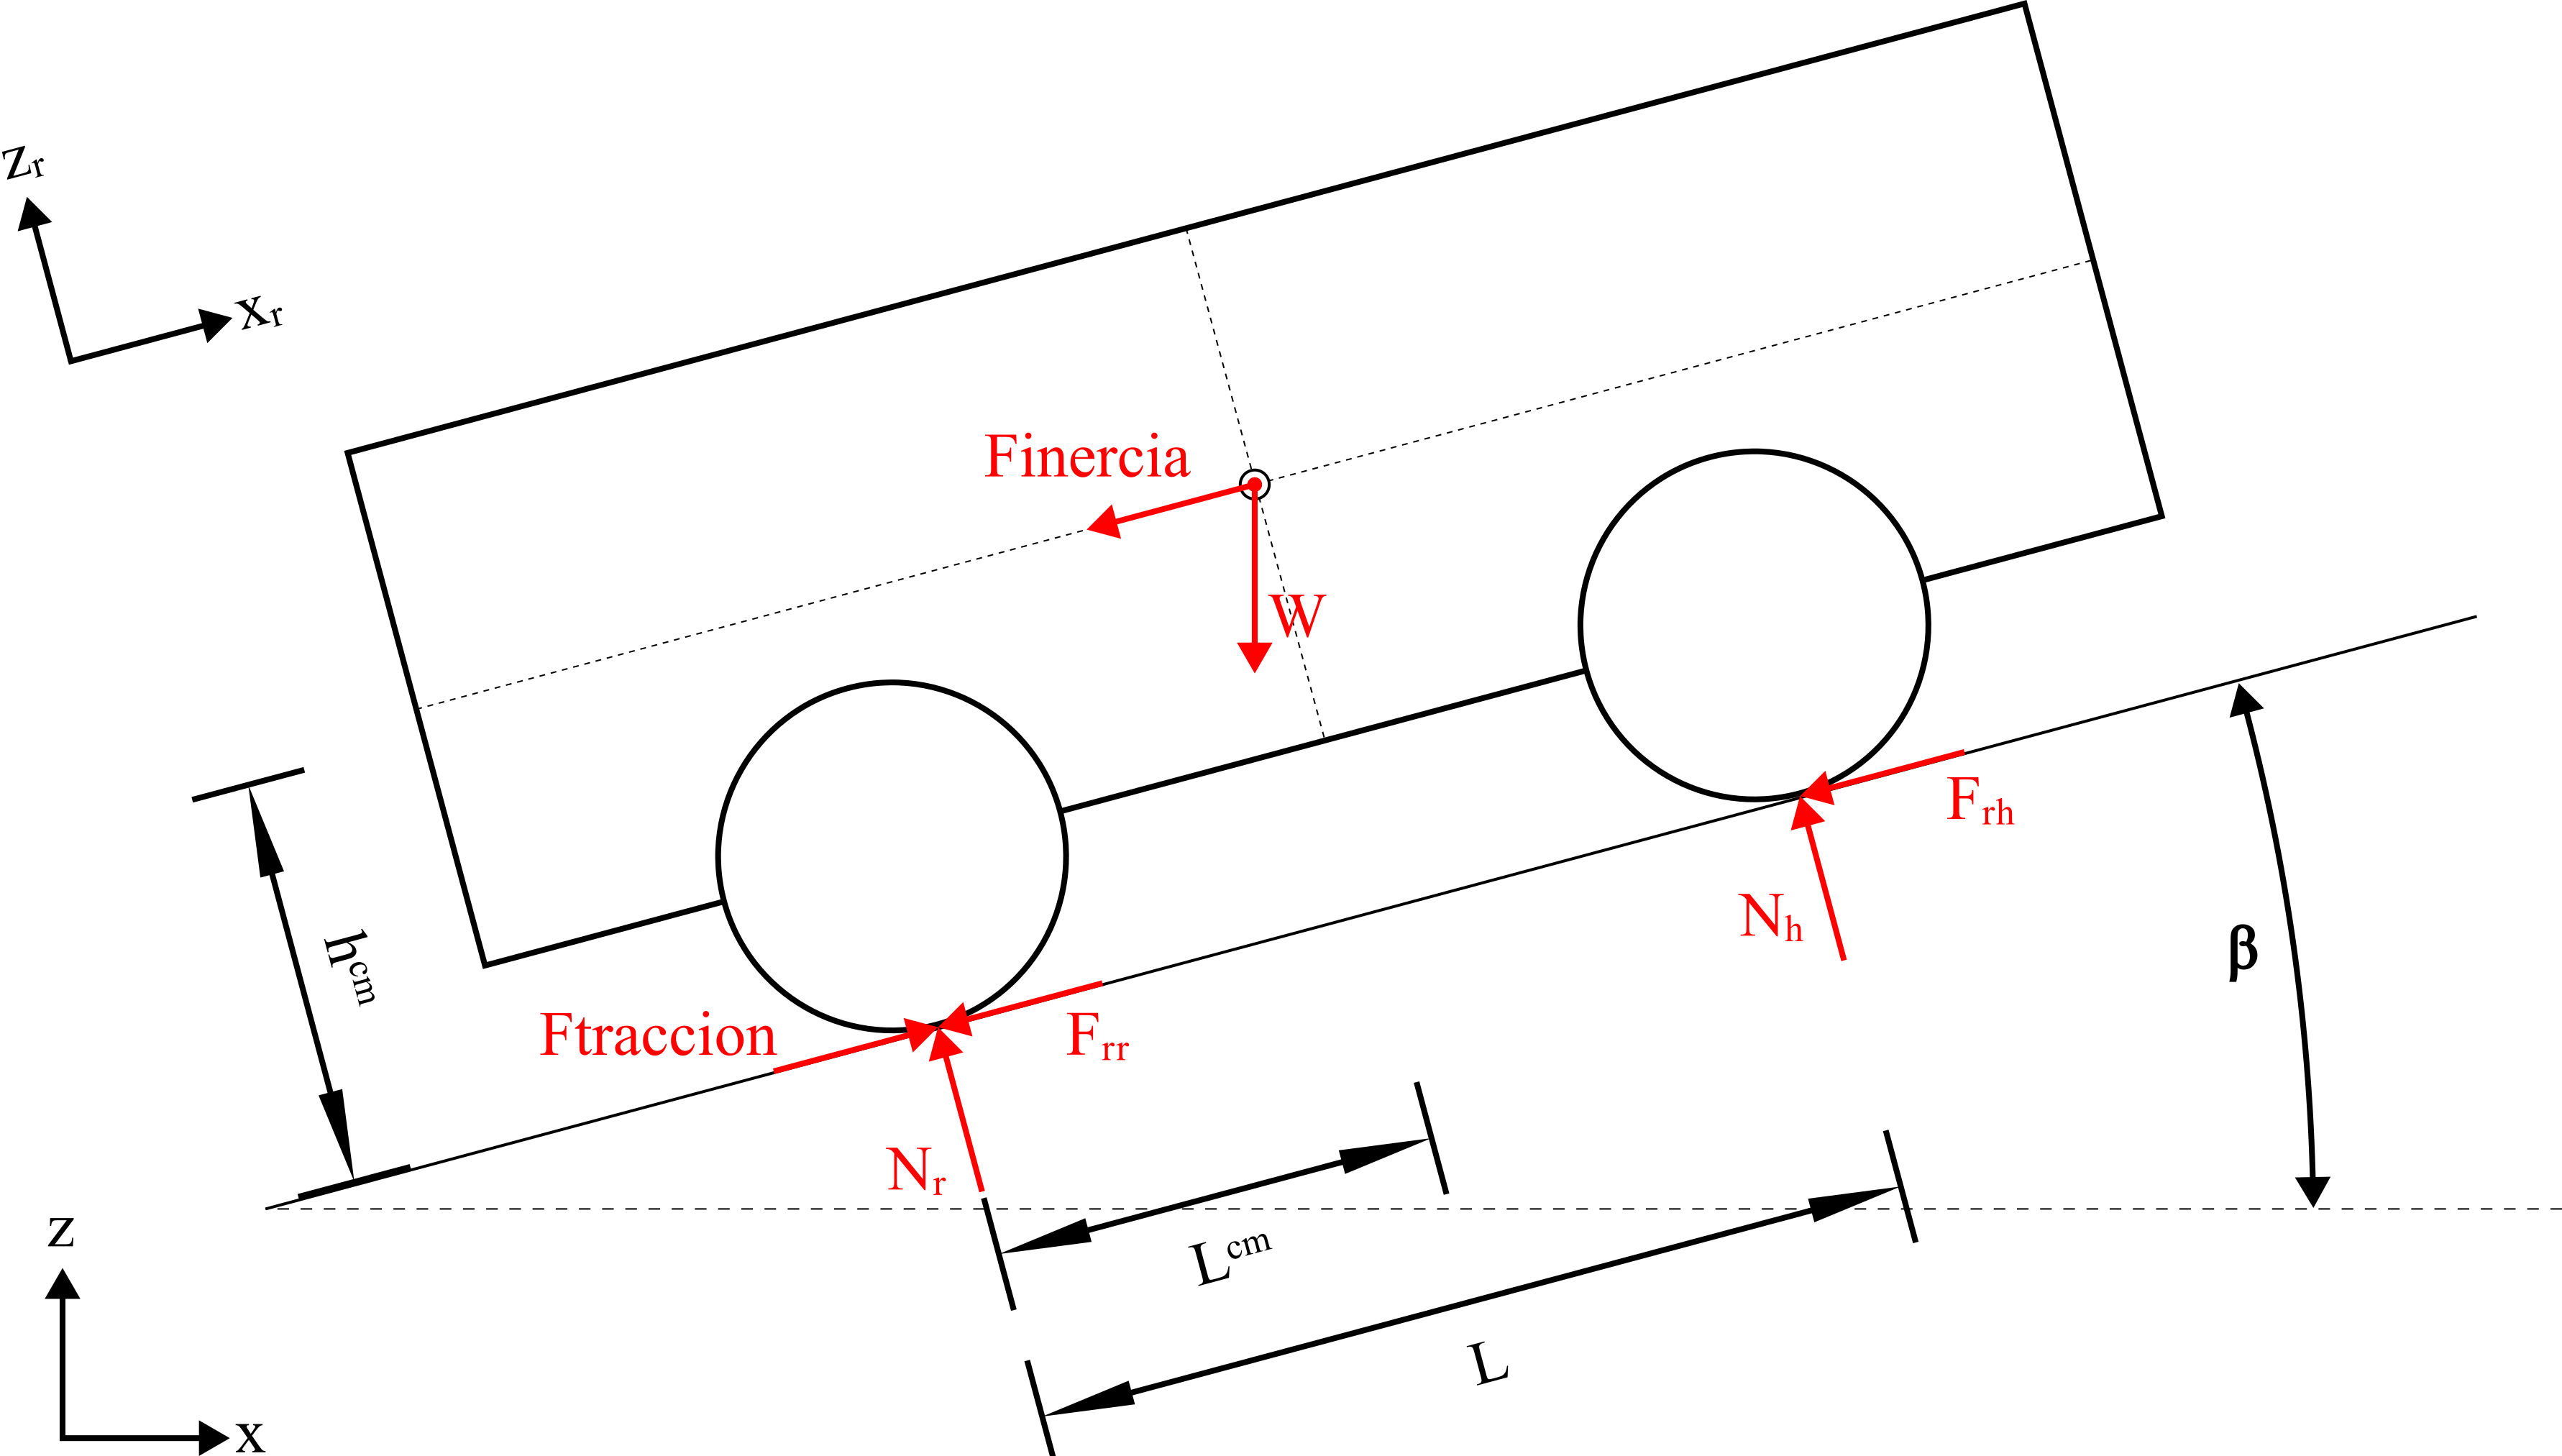
\includegraphics[width=0.75\textwidth]{Recursos/Imagenes/ImagenesDisenoMecanico/Trac_DCL.png} \par\medskip
	
	\raggedright
	\footnotesize \textit{Nota.} Elaboración propia.
	\label{fig:DCLSubsistemaTraccion}
\end{figure}

\begin{figure}[H]
	\captionsetup{justification=raggedright, singlelinecheck=false, labelsep=none}
	
	\caption[Diagrama de cuerpo libre de movimiento del subsistema de dirección.]{} 
	
	\textit{Diagrama de cuerpo libre de movimiento del subsistema de dirección.} \par\medskip
	
	\centering
	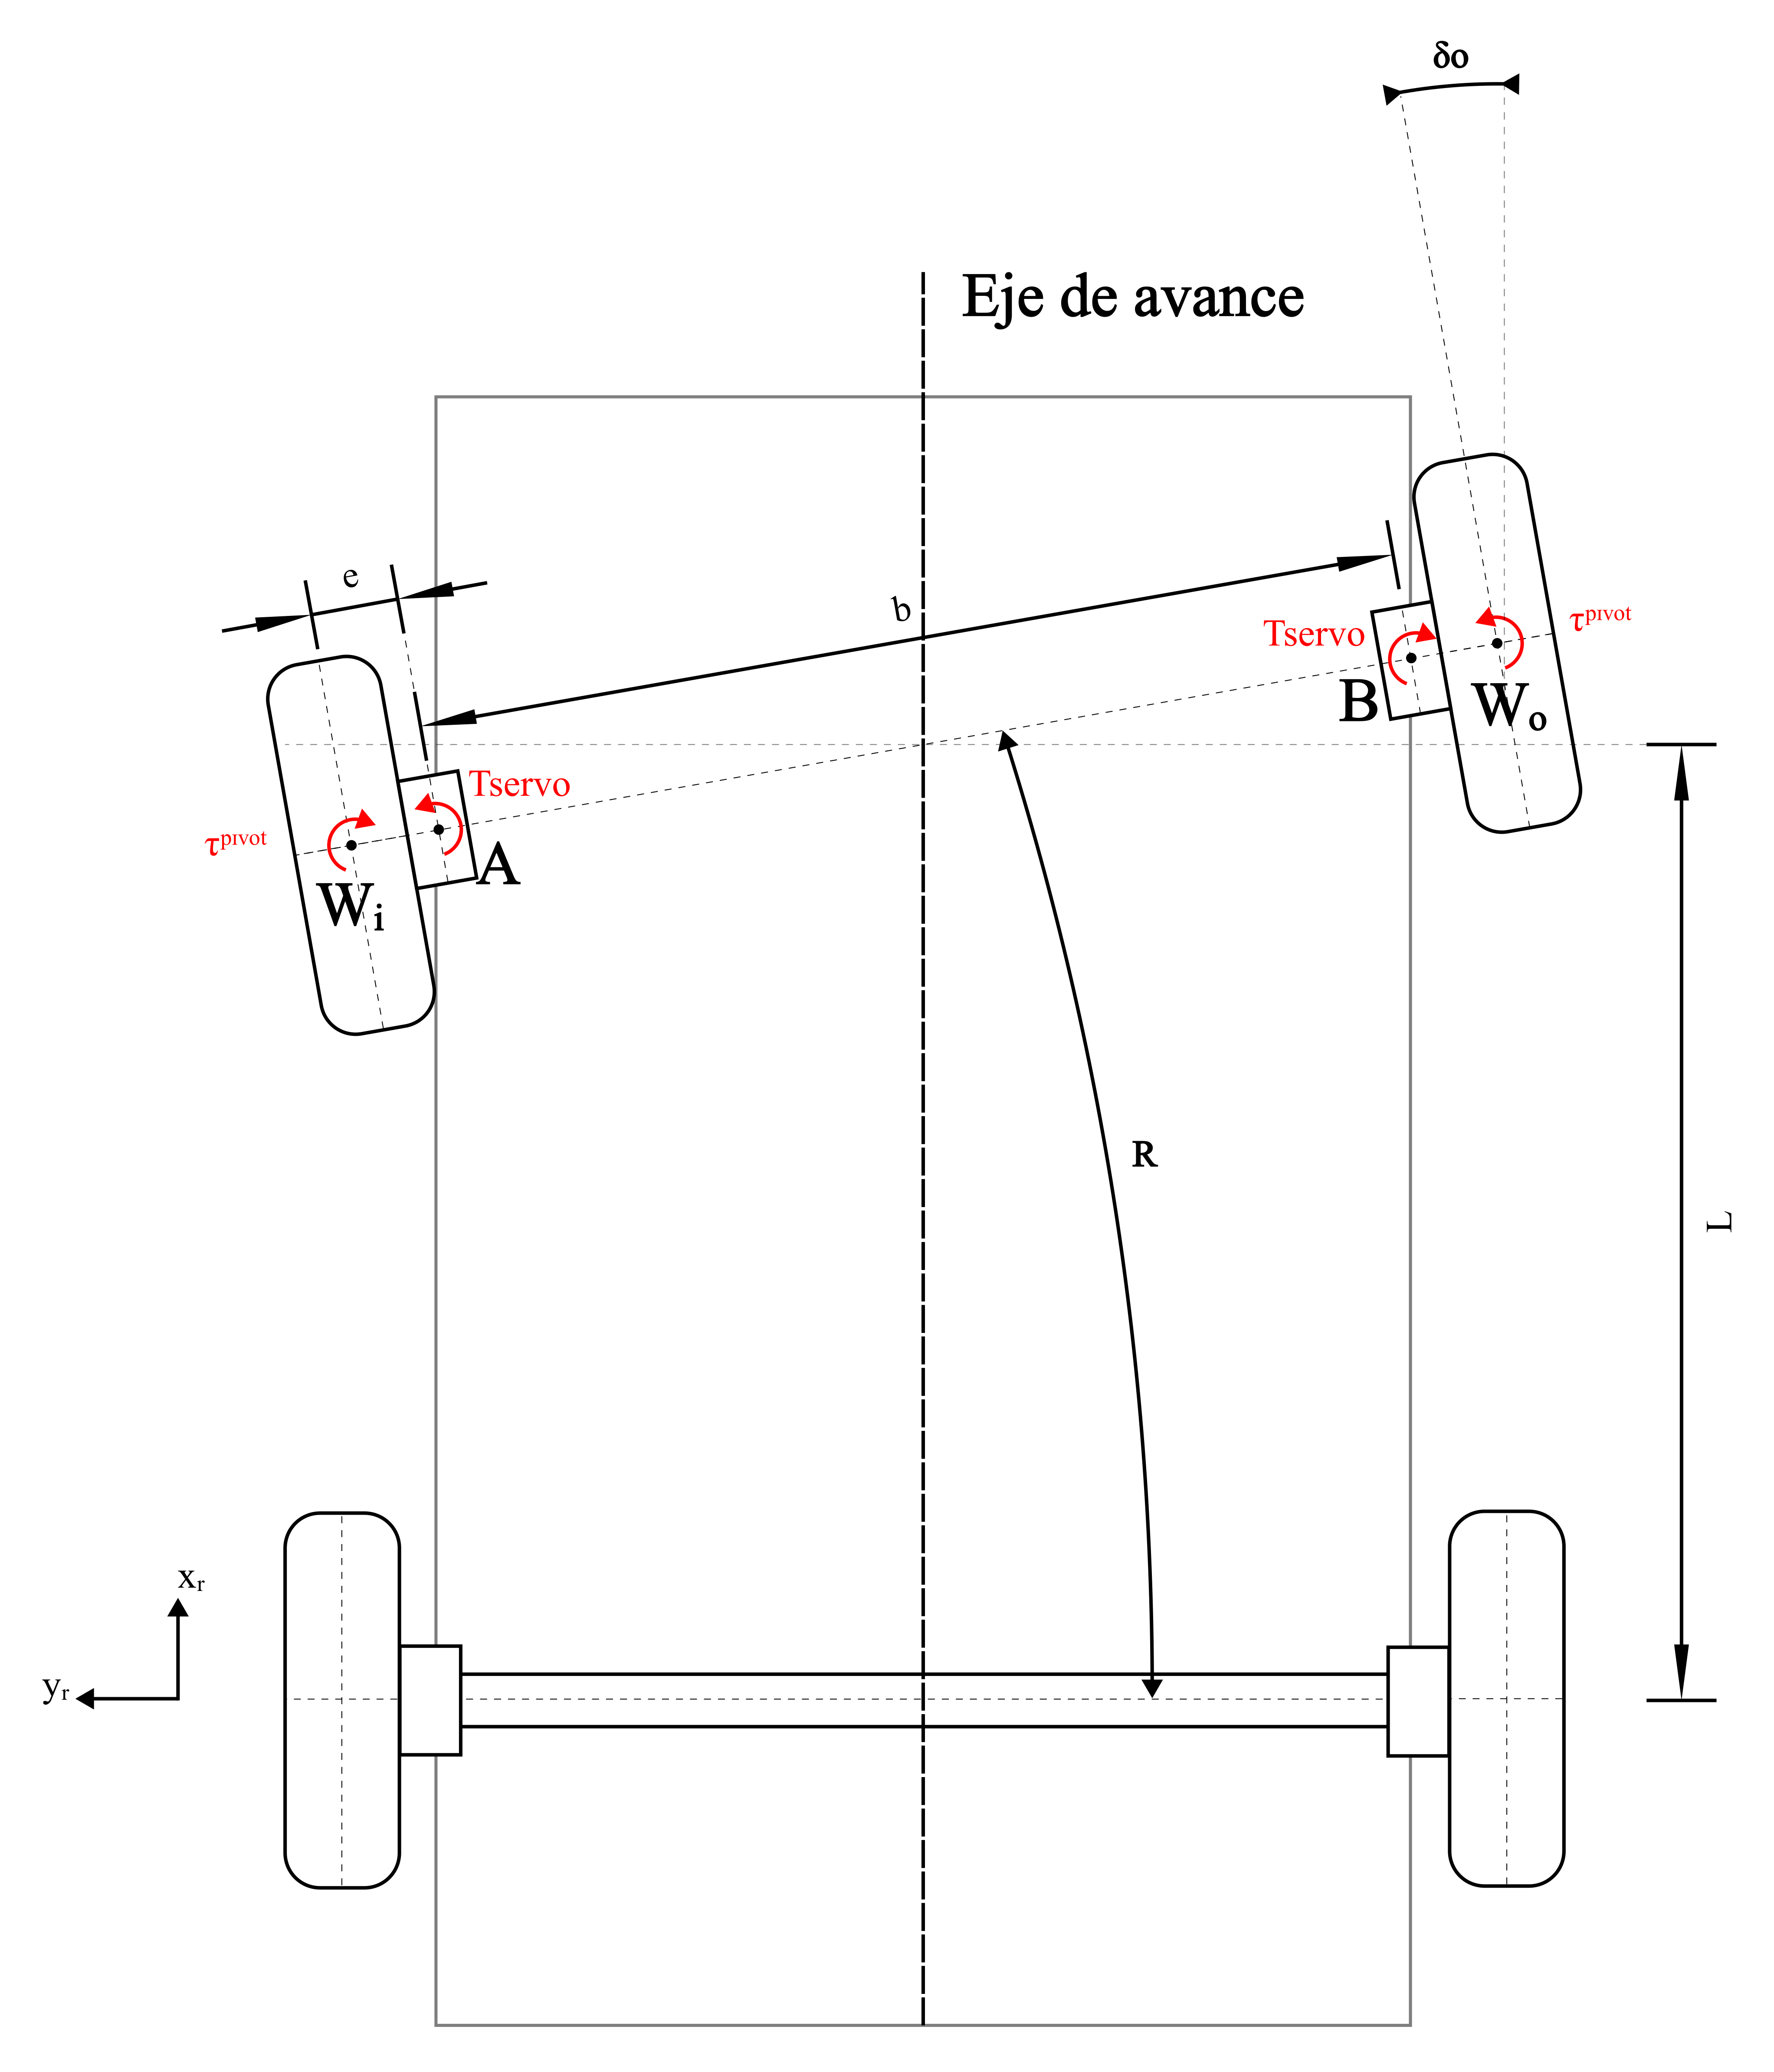
\includegraphics[width=0.75\textwidth]{Recursos/Imagenes/ImagenesDisenoMecanico/Dir_DCL.png} \par\medskip
	
	\raggedright
	\footnotesize \textit{Nota.} Elaboración propia.
	\label{fig:DCLSubsistemaDireccion}
\end{figure}

El análisis dinámico se divide en un plano longitudinal de elevación para la tracción y en el plano horizontal de marcha para la dirección.

A partir del equilibrio longitudinal, la fuerza de resistencia a la rodadura total dependiente de la inclinación del terreno $\beta$ se expresa como:

\begin{equation*}
    F_{rr,\text{total}} = f_r \cdot m \cdot g \cdot \cos \beta
\end{equation*}

A partir de la Segunda Ley de Newton aplicada al centro de gravedad del vehículo en la vista lateral, el robot que asciende por una pendiente de inclinación $\beta$ experimenta tres fuerzas opuestas al movimiento, correspondientes a la componente gravitacional paralela a la rampa, la resistencia a la rodadura total de los neumáticos y la fuerza inercial por aceleración. La fuerza de tracción tangencial $F_{\text{trac}}$ ejercida por las ruedas posteriores debe ser numéricamente igual a la suma de estos tres componentes:

\begin{equation*}
    F_{\text{trac}} = m \cdot a + m \cdot g \cdot \sin \beta + F_{rr,\text{total}}
\end{equation*}

Del equilibrio de fuerzas normales, la carga normal total corresponde al coseno del ángulo multiplicado por el peso. La distribución de carga sobre el eje frontal por transferencia de peso se obtiene resolviendo momentos respecto al apoyo posterior:

\begin{equation*}
    N_f = \frac{m \cdot g \cdot \cos \beta \cdot L_{cm} - m \cdot g \cdot \sin \beta \cdot h_{cm} - m \cdot a \cdot h_{cm}}{L}
\end{equation*}

La carga normal sobre el eje posterior corresponde a la resta entre la carga total y la frontal.

Considerando el radio de rueda $r$, la relación de transmisión $i_t$, la eficiencia $\eta_t$ y el factor de seguridad $S$, el torque continuo en el motorreductor de tracción es:

\begin{equation*}
    T_{\text{motor},t} = \frac{F_{\text{trac}} \cdot r \cdot S}{i_t \cdot \eta_t}
\end{equation*}

Para garantizar que la fuerza de tracción requerida se transmita efectivamente al suelo sin que las ruedas motrices patinen, se impone la restricción de adherencia estática de Coulomb. La carga normal sobre el eje posterior incluye la redistribución dinámica de peso debida a la inclinación del terreno y a la aceleración del vehículo:

\begin{equation*}
    F_{\text{trac}} \le \mu_s \cdot N_r
\end{equation*}

Para el subsistema de dirección accionado por doble servomotor, el torque de resistencia al pivoteo por mangueta, conocido como scrub torque \citep{jazar2017vehicle}, con carga normal por rueda delantera resulta en:

\begin{equation*}
    \tau_{\text{piv}} = \frac{2}{3} \cdot \mu_s \cdot N_{\text{rueda}_f} \cdot r_c + \mu_s \cdot N_{\text{rueda}_f} \cdot e
\end{equation*}

Al emplear un esquema de dirección electrónica independiente, cada mangueta delantera es accionada por su propio servomotor acoplado coaxialmente al pivote vertical. Por lo tanto, el torque demandado individualmente no requiere ser dividido entre dos, sino que debe vencer de forma directa el torque de frotamiento. Este último se origina por la fricción de pivoteo de la huella de contacto del neumático al girar sobre un punto desfasado una distancia transversal respecto al eje. Considerando la relación de transmisión, la eficiencia y el factor de seguridad, el torque por servomotor es:

\begin{equation*}
    T_{\text{servo}} = \frac{\tau_{\text{piv}} \cdot S}{i_s \cdot \eta_s}
\end{equation*}

Añadiendo la inercia rotacional de las ruedas y componentes giratorios junto al torque de fricción estática inicial en el tren motriz, el torque motor total de tracción requerido durante el movimiento de despegue se expresa como:

\begin{equation*}
    T_{\text{motor},t,\text{total}} = \frac{\left[ F_{\text{trac}} \cdot r + J_{\text{ruedas}} \cdot \frac{a}{r} \right] \cdot S}{i_t \cdot \eta_t} + T_{s,t}
\end{equation*}

Para la dirección, considerando la inercia de la mangueta, la aceleración angular de viraje y el rozamiento de despegue, el par máximo por servomotor individual durante el movimiento es:

\begin{equation*}
    T_{\text{servo},\text{total}} = \frac{\left[ \tau_{\text{piv}} + J_{\text{mang}} \cdot \ddot{\delta} \right] \cdot S}{i_s \cdot \eta_s} + T_{s,s}
\end{equation*}

\subsection{Dimensionamiento de componentes}

El análisis en el plano longitudinal ejecutado sobre una pendiente máxima de ascenso de $15^\circ$ para la masa nominal estipulada de $17.50\text{ kg}$ revela una resistencia de componente gravitacional igual a $44.43\text{ N}$, que sumada a una resistencia a la rodadura de $9.95\text{ N}$, exige una demanda de fuerza tangencial continua de $54.38\text{ N}$. Durante la fase inicial de despegue, asumiendo una aceleración constante, la fuerza pico solicitada asciende a $63.13\text{ N}$. La verificación del criterio de adherencia de Coulomb certifica rigurosamente que, con una transferencia dinámica de masa que ubica una carga de $104.18\text{ N}$ sobre el eje posterior, y empleando un coeficiente estático para llantas de caucho sobre terreno suelto de $0.70$ \citep{wong2022ground}, el límite traccional sin patinamiento es de $72.92\text{ N}$, superando el empuje inercial requerido. Trasladando esta demanda tangencial a un torque en los neumáticos, los cuales poseen un diámetro externo perimetral de $200\text{ mm}$, se precisa una fuerza torsional en el eje principal continuo de $6.31\text{ N}\cdot\text{m}$. Absorbiendo las pérdidas por rendimiento de transmisión mediante un factor de 0.85, el actuador de corriente directa está supeditado a entregar un par límite de $9.65\text{ N}\cdot\text{m}$.

En el régimen cinemático rotacional a una velocidad sostenida de marcha de $1.0\text{ m/s}$, el tren de tracción gira a $95.5\text{ RPM}$, lo que exige una provisión de potencia mecánica de $54.4\text{ W}$. Operando a través del bus de potencia a un voltaje directo de $24\text{ V}$, este requerimiento dinámico se traduce en una absorción eléctrica nominal de corriente en el rango de los $2.67\text{ A}$. El módulo electrónico de gobierno del motor, materializado en el puente H dual de referencia BTS7960 capacitado para una corriente umbral de $43\text{ A}$, domina este parámetro eléctrico operando bajo un grado de seguridad y tolerancia térmica superior a 9.0, garantizando una temperatura de transición sumamente contenida.

A nivel de estructuración y dimensionamiento mecánico de chasis, el eje motriz debe sostener en servicio un esfuerzo equivalente combinado de Von Mises \citep{Shigley11th} definido en $6.73\text{ N}\cdot\text{m}$, proveniente de la flexión en los apoyos de voladizo y el par torsor que lo surca. El análisis arrojó un diámetro admisible base para el acero calibrado AISI 1045 con un factor de seguridad generalizado de 3.0 igual a $8.72\text{ mm}$. Al adoptar normativamente un macizo torneado comercial de una cota equivalente a $12.0\text{ mm}$ con tolerancia h6 \citep{iso286_2_2010}, se absorben los cambios por deformación. El anclaje de este eje corre a cargo de rodamientos axiales SKF 6001-2RSH, cuyas capacidades dinámicas alcanzan los $5.40\text{ kN}$ frente al impacto de $0.33\text{ kN}$ recibido en pista, perpetuando su expectativa de vida por encima de los ciclos mecánicos programados. En la arquitectura de dirección, el par torsional de pivoteo de la mangueta en contacto con el suelo requiere del suministro de $14.01\text{ kg}\cdot\text{cm}$ de fuerza rotativa. Para esto se implementan los potentes servomotores individuales RDS3225, evaluados en $25.0\text{ kg}\cdot\text{cm}$, que brindan al mecanismo un respaldo resolutivo con un factor de estabilidad del 1.78 bajo estricto servicio de viraje en tramas agrestes. Las espigas directrices frontales, torneadas en acero a $10.0\text{ mm}$ y ancladas a las manguetas de aluminio estructural 6061-T6, y los pasadores verticales de pivotación tipo kingpin con diámetros de $8.0\text{ mm}$, trabajan frente al esfuerzo de cortadura pura bajo márgenes centuplicados.

Para el enlace cinemático entre el motorreductor y el eje posterior, la transmisión síncrona por correa dentada se dimensiona adoptando un factor de servicio de sobrecarga $K_s = 1.50$, lo que eleva el par de diseño nominal a $12.48\text{ N}\cdot\text{m}$ y el par pico de arranque en rampa a $14.48\text{ N}\cdot\text{m}$. A la velocidad de giro de $95.5\text{ RPM}$ sobre una polea motriz de $24$ dientes con diámetro de paso de $38.20\text{ mm}$, la fuerza tangencial efectiva de diseño alcanza $653.45\text{ N}$. Esta demanda queda cubierta con holgura frente a la capacidad de carga permisible de la correa ($850\text{ N}$) y su resistencia de rotura por tracción ($3200\text{ N}$), asegurando un factor de seguridad de 1.30 ante saltos de dientes durante el arranque. La tensión inicial de instalación por ramal se calibra en $490.1\text{ N}$, verificable en banco mediante una deflexión de $2.16\text{ mm}$ bajo la aplicación de una carga perpendicular de prueba de $28.0\text{ N}$ en el centro del tramo libre de $135.0\text{ mm}$. La fuerza radial resultante transmitida hacia los ejes de $980.2\text{ N}$ es absorbida de forma compartida por los rodamientos SKF 6001-2RSH ($C_0 = 2.36\text{ kN}$), confiriendo un factor de seguridad estático de $2.41$ y asegurando una vida nominal libre de fallas superior a 100000 horas de servicio \citep{iso281_2007}.

\subsection{Selección de componentes}

\subsubsection{Selección del motorreductor de tracción posterior}

Las demandas dinámicas exigen que el actuador provea una fuerza continua en rampa de 15 grados evaluada en 54.38 N, con un pico de despegue de 63.13 N. A una velocidad nominal de avance de 1.0 m/s, que equivale a 95.5 RPM en ruedas con diámetro de 200 mm, se requiere un torque motor continuo igual o superior a 8.32 N m.

Se evalúan tres alternativas comerciales de motorreductores operando a un voltaje directo de 24 V. La Opción A es un motorreductor planetario de 60 W de potencia. La Opción B es un motorreductor de corriente directa de alta potencia con 80 W e incluye un tren de engranajes cilíndricos templados. La Opción C plantea el acople de un motor de 90 W a un reductor de tipo sinfín y corona modelo NMRV030.

\begin{center}
    \footnotesize
    \begin{xltabular}{\textwidth}{|p{3.5cm}|>{\centering\arraybackslash}X|>{\centering\arraybackslash}X|>{\centering\arraybackslash}X|}
        \caption{Tabla comparativa de motorreductores de tracción evaluados\label{tab:comp_motorreductores}} \\
        \hline
        \rowcolor[HTML]{D9E1F2} 
        Especificación Técnica & Opción A Planetario 60W & Opción B Engranes 80W & Opción C NMRV030 90W \\ \hline
        \endfirsthead
        
        \multicolumn{4}{c}%
        {\tablename\ \thetable{} -- Continuación de la página anterior} \\
        \hline
        \rowcolor[HTML]{D9E1F2} 
        Especificación Técnica & Opción A Planetario 60W & Opción B Engranes 80W & Opción C NMRV030 90W \\ \hline
        \endhead
        
        \hline
        \endfoot
        
        \hline
        \endlastfoot
        
        Tensión de Operación & $24\text{ V DC}$ & $24\text{ V DC}$ & $24\text{ V DC}$ \\ \hline
        Velocidad en Carga & $80\text{ RPM}$ & $96\text{ RPM}$ & $100\text{ RPM}$ \\ \hline
        Torque Nominal Continuo & $6.0\text{ N}\cdot\text{m}$ & $10.0\text{ N}\cdot\text{m}$ & $12.0\text{ N}\cdot\text{m}$ \\ \hline
        Torque de Bloqueo & No evaluado & $25.0\text{ N}\cdot\text{m}$ & No aplicable \\ \hline
        Corriente Nominal & No evaluada & $3.33\text{ A}$ & Excesiva \\ \hline
        Masa Total & $1.45\text{ kg}$ & $1.35\text{ kg}$ & $2.20\text{ kg}$ \\ \hline
    \end{xltabular}
\end{center}

Se selecciona la Opción B correspondiente al motorreductor de 80 W, ya que otorga un margen de torque seguro con un factor de 1.20 frente a la demanda de 8.32 N m, logrando una velocidad de avance de 1.01 m/s. Además, presenta compatibilidad directa con el driver tipo Puente H Dual BTS7960, cuya enorme capacidad de 43 A excede holgadamente la corriente nominal de 3.33 A. La Opción A resulta insuficiente en par de rampa, mientras que la Opción C impone una penalización de peso del 63 por ciento y un autobloqueo excesivo que impide el empuje manual en situaciones de emergencia.

\subsubsection{Selección de la transmisión por correa dentada}

Para garantizar una transmisión de potencia síncrona, silenciosa y exenta de lubricación ante la presencia de polvo y grava, se selecciona una correa dentada de perfil curvilíneo HTD 5M (o S5M) con paso de $5.0\text{ mm}$ y un ancho nominal estandarizado de $15.0\text{ mm}$ \citep{iso13050_2014}, provista de cuerdas de tracción internas de fibra de vidrio. La geometría curvilínea optimiza la distribución de tensiones en la base de los dientes, eliminando puntos de concentración de carga y permitiendo absorber los picos de arranque en pendiente sin deslizamiento.

El tren síncrono adopta poleas comerciales de aluminio de $24$ dientes ($Z_d = Z_D = 24$) con un diámetro de paso de $38.20\text{ mm}$ y un diámetro exterior de $37.24\text{ mm}$, estableciendo una relación de transmisión directa de uno a uno ($1:1$). Para una distancia entre centros nominal de $135.0\text{ mm}$, el arco de contacto en ambas poleas alcanza los $180^\circ$, manteniendo $12$ dientes en engrane simultáneo, lo cual asegura el aprovechamiento íntegro de la capacidad nominal de la correa ($K_m = 1.0$). En función de estos parámetros geométricos, se adopta la longitud comercial HTD 5M-390 con $390.0\text{ mm}$ de longitud de paso y $78$ dientes totales. Para impedir el desplazamiento lateral (\textit{tracking}) de la correa por cargas parásitas, la polea del motorreductor dispone de pestañas de retención lateral (\textit{flanges}) en ambos costados, facilitando el montaje del motor sobre correderas con ranuras colisas para graduar la distancia entre centros y asegurar una alineación angular estricta menor o igual a $0.25^\circ$.

\subsubsection{Selección del eje posterior rígido y acoplamiento mecánico}

El eje posterior rígido de tipo \textit{Live Axle} se diseña a partir de una barra maciza de acero al carbono AISI 1045 rectificada bajo tolerancia h6 \citep{iso286_2_2010}, con un diámetro de $12.0\text{ mm}$ y una longitud total de $490\text{ mm}$. Para el acople a torsión entre las poleas dentadas y los ejes (tanto en la salida del motorreductor como en el eje posterior), se mecanizan mandriles centrales a $\phi\,12.0\text{ mm}$ con tolerancia H7 \citep{iso286_2_2010} y chaveteros normalizados bajo el estándar DIN 6885-A \citep{din6885_1}. La unión se concreta mediante chavetas paralelas de lengüeta de $4 \times 4 \times 25\text{ mm}$ en acero C45. Ante el par pico de diseño de $14.48\text{ N}\cdot\text{m}$, la fuerza tangencial en la chaveta de $2413.3\text{ N}$ induce un esfuerzo cortante de $24.13\text{ MPa}$ y un esfuerzo de aplastamiento de $48.27\text{ MPa}$; ambos valores se sitúan ampliamente por debajo de las resistencias admisibles del material ($119.2\text{ MPa}$ y $206.7\text{ MPa}$, respectivamente), consolidando factores de seguridad de $4.94$ al corte y $4.28$ al aplastamiento. La inmovilización axial se completa mediante dos prisioneros roscados M5 a $90^\circ$ sobre el cubo de cada polea.

\subsubsection{Selección de soportes y chumaceras de eje motriz}
El montaje y giro libre del eje de tracción se resuelve con la selección de dos chumaceras bridadas ovaladas de dos pernos tipo KFL001, las cuales alojan internamente rodamientos rígidos de bolas SKF 6001-2RSH de 12 por 28 por 8 mm provistos de doble sello de caucho. El diseño exige obligatoriamente un montaje debajo de la viga inferior del chasis, configuración que permite a las chumaceras trabajar a compresión directa sobre la estructura de aluminio, protegiendo los pernos tensores M5 y asegurando un despeje libre desde el suelo de 100 mm. La vida útil nominal calculada supera las 100000 horas continuas \citep{iso281_2007}.

\subsubsection{Selección de neumáticos, rines y cubos de rueda posteriores}
Se incorporan neumáticos de caucho con diseño todo terreno, presentando un diámetro exterior de 200 mm y un ancho de huella variable entre 50 y 55 mm, los cuales se montan sobre rines de aluminio de 100 mm de diámetro. La transmisión de potencia hacia los rines se concreta mediante cubos de rueda mecanizados en aluminio 6061-T6, dotados con un ajuste H7 que abraza el eje de 12 mm e incorpora chavetero de 4 mm bloqueado con tornillos prisioneros M5.

\subsubsection{Selección del acople y soporte del encoder de odometría}
La retroalimentación posicional del tren posterior se instrumenta instalando un encoder rotativo óptico incremental de cuadratura Omron E6B2-CWZ6C, el cual genera 1000 pulsos por revolución y opera salidas NPN a 5 V. La conexión física al eje de tracción se realiza utilizando un acople elástico helicoidal de aluminio reductor de 12 mm a 6 mm, mientras que el cuerpo del sensor se inmoviliza a la estructura mediante un soporte de chapa de aluminio configurado a medida.

\subsubsection{Selección del actuador de dirección}

El requerimiento base de par resistente al pivoteo en reposo fue cuantificado en 0.951 N m, escalando a 1.09 N m en condiciones críticas. Incorporando el factor de seguridad estructural de 1.30, el par mínimo demandado alcanza 1.374 N m, valor que se traduce a 14.01 kg cm. Como criterios adicionales se establece alimentación a 7.4 V directos desde un bus de energía dedicado, piñonería metálica y un grado de protección envolvente IP66.

Se contrastan tres ofertas en el segmento de servomotores de alto torque. La Opción A recae en el modelo digital RDS3225 fabricado por Dsservo. La Opción B analiza el modelo Savöx SW-0231MG. Finalmente, la Opción C evalúa el desempeño del componente FEETECH FS5115M.

\begin{center}
    \footnotesize
    \begin{xltabular}{\textwidth}{|p{3.5cm}|>{\centering\arraybackslash}X|>{\centering\arraybackslash}X|>{\centering\arraybackslash}X|}
        \caption{Tabla comparativa de servomotores de dirección evaluados\label{tab:comp_servomotores}} \\
        \hline
        \rowcolor[HTML]{D9E1F2} 
        Especificación Técnica & Opción A RDS3225 & Opción B Savöx SW-0231MG & Opción C FEETECH FS5115M \\ \hline
        \endfirsthead
        
        \multicolumn{4}{c}%
        {\tablename\ \thetable{} -- Continuación de la página anterior} \\
        \hline
        \rowcolor[HTML]{D9E1F2} 
        Especificación Técnica & Opción A RDS3225 & Opción B Savöx SW-0231MG & Opción C FEETECH FS5115M \\ \hline
        \endhead
        
        \hline
        \endfoot
        
        \hline
        \endlastfoot
        
        Torque Nominal & $25.0\text{ kg}\cdot\text{cm}$ a 7.4V & $15.0\text{ kg}\cdot\text{cm}$ a 6.0V & $15.5\text{ kg}\cdot\text{cm}$ a 7.4V \\ \hline
        Material de Piñones & Cobre y Aluminio mecanizado & Acero y Aluminio & Cobre \\ \hline
        Grado de Protección & Estanco IP66 & Estanco IP67 & No estanco IP54 \\ \hline
        Masa del Componente & $60.0\text{ g}$ & $66.0\text{ g}$ & $58.0\text{ g}$ \\ \hline
        Factor de Seguridad & $1.78$ & $1.07$ & Insuficiente en polvo \\ \hline
    \end{xltabular}
\end{center}

Se escoge de forma definitiva la Opción A con el modelo RDS3225, justificado principalmente por su amplio margen de torque, el cual entrega un factor de seguridad de 1.78 sobre la exigencia de 14.01 kg cm. Además, sobresale por la composición de sus piñones en cobre y aluminio mecanizados, la incorporación de un doble rodamiento de bolas para fluidez, y su envolvente con grado IP66 estanca contra arena y agua. Este modelo soporta barridos angulares entre 180 y 270 grados. Las otras opciones o bien presentan factores de seguridad ajustados ante picos de resistencia en grava, o adolecen de riesgo por penetración de polvo en el potenciómetro interno.

\subsubsection{Selección y verificación de las manguetas de dirección}
El elemento vinculante central de la dirección se concreta mediante el diseño de una horquilla en forma de C mecanizada íntegramente en placa de aluminio 6061-T6 con un espesor sólido de 6.0 mm. La prolongación geométrica de este componente establece un brazo de palanca operativo de 30 mm, el cual fue validado exitosamente ante ensayos de flexión sobre su estructura y las orejas de fijación sin reportar deformación permanente.

\subsubsection{Selección de la espiga horizontal y rodamientos de rueda delantera}
La masa soportada por los neumáticos directrices se transfiere a través de una espiga de acero calibrado AISI 1045 rectificada bajo tolerancia h6, con un diámetro de 10.0 mm y una longitud de 45 mm, rematada con una rosca de sujeción macho M10 de paso fino. La comprobación analítica del momento flector de 1.93 N m determina un diámetro mínimo seguro de 5.75 mm, por lo que la elección de la cota de 10.0 mm concede un aplastante factor de seguridad de 5.26. La espiga transita libremente apoyada por dos rodamientos rígidos SKF 6000-2RSH de 10 por 26 por 8 mm por cada rueda, garantizando una vida útil libre de fricción que excede las 100000 horas. Al emplear neumáticos frontales del mismo diámetro que los posteriores, de 200 mm, se mantiene el chasis perfectamente nivelado a 100 mm de altura y se asegura el ángulo de ataque idóneo en terrenos con grava.

\subsubsection{Selección de los pasadores de pivote vertical y bujes}
El anclaje del viraje direccional tipo kingpin se efectúa utilizando un pasador rectificado fabricado en acero AISI 1045 de 8.0 mm de diámetro. El análisis revela que este elemento labora sometido a esfuerzos de corte doble, exhibiendo una fatiga de tan solo 0.43 MPa frente al abismal límite del material cifrado en 140 MPa. La transición suave de los movimientos rotacionales queda a cargo de dos bujes de bronce sinterizado autolubricante tipo SAE 660, con dimensiones de 8 por 12 por 8 mm instalados en cada mangueta, erradicando holguras perjudiciales.

\subsubsection{Mecanismo de articulación y bieletas de transmisión}
El enlace mecánico entre la hornilla dentada del servomotor y la mangueta orientable se forja empleando varilla roscada M4 de acero de alta dureza, cuyos extremos se equipan con terminales esféricos de rótula autolubricante Rod Ends. Esta arquitectura de eslabonamientos provee una transmisión fiel con relación directa y exenta del juego mecánico, acoplando instantáneamente la directriz trazada desde el brazo de 25 dientes del actuador hacia la rueda.

\subsection{Simulación y validación}

\end{document}
